\documentclass{beamer}
\usecolortheme{wolverine}

% math stuff
\usepackage{amsmath}
\usepackage{amsthm}
\usepackage{amssymb}
\usepackage{xcolor}

\usepackage{float}
\usepackage{subcaption}

% to insert images
\usepackage{graphicx}

% to correctly insert stressed characters
\usepackage[T1]{fontenc}
\usepackage[utf8]{inputenc}

\usepackage{multirow}

% Bibliography
% \usepackage[style=alphabetic]{biblatex}
% \usepackage[nottoc]{tocbibind}
% \usepackage{bibentry}
% \setcounter{biburllcpenalty}{9000}
% \usepackage{nameref}
% \addbibresource{slides.bib}

% to put links in table of contents
\usepackage{hyperref}
\hypersetup{colorlinks=false, %set true if you want colored links
	linktoc=all,     %set to all if you
}

\usepackage{mathtools}

% Add symbols
% \usepackage{textcomp}

% Add command for Real and Z sets
% \usepackage{dsfont}
% \newcommand{\Rset}{$\mathds{R}$}
% \newcommand{\Zset}{$\mathds{Z}$}

% Code highlighting
% \usepackage{minted}
% \usemintedstyle{perldoc}
% \setminted{
%     frame=single,
%     breaklines,
% }

% tikz figures
% \usepackage{tikzit}
% \input{style.tikzstyles}

% number rounding
\usepackage{siunitx}
\sisetup{round-mode=places,round-precision=5}

\definecolor{myyellow}{RGB}{225, 225, 0}

\title{Thesis notes}
\date{27th April}

% any code between @(...)@ is escaped back to LaTeX
% \lstset{escapeinside={@(}{)@}}

% algorithms
\usepackage[ruled,vlined]{algorithm2e}
% \newtheorem{theorem}{Theorem}

\begin{document}

\frame{\titlepage}

\begin{frame}[c]
	\frametitle{The Echo Chamber Problem - notation}

	\begin{itemize}
		\item $G = (V, E ^{+}, E ^{-}) $ interaction graph
		\item $ \mathcal{C} $ set of contents
		\item $C \in \mathcal{C} $ content, $\mathcal{T} _{C} $ set of threads
		      associated with $C$. A thread $T \in \mathcal{T} _{C} $ is a
		      subgraph of $G$
		      % So $G = \bigcup _{C
		      % \in \mathcal{C} } \bigcup _{T \in \mathcal{T} _C} T $ union of all
		      % threads of all contents
		\item $U \subseteq V$ subset of users, $T[U]$ subgraph of $T$ induced
		      by $U$. $|T(U)|$ is the number of edges of this subgraph
	\end{itemize}
\end{frame}

\begin{frame}[c]
	\frametitle{The Echo Chamber Problem - notation}
	\begin{itemize}
		\item $\eta(C)$ fraction of negative edges associated with $C$
		      (analogous definition for a thread $T$). Content (or thread)
		      controversial if $\eta \in [\alpha, 1]$
		\item $\hat{\mathcal{C} } \subseteq \mathcal{C} $ set of \textit{controversial}
		      contents

		\item $\mathcal{S} _C (U)$ set of \textit{non controversial} threads
		      induced by $U$, for \textit{controversial} contents, i.e.

			      {\small
				      \begin{equation}
					      \mathcal{S} _{C} (U) = \{ T[U] \; s.t. \; T[U] \; non \;
					      controversial, T \in \mathcal{T} _{C}, C
					      \in \hat{\mathcal{C}}, U \subseteq V\}
				      \end{equation}
			      }
	\end{itemize}

\end{frame}

\begin{frame}[c]
	\frametitle{The Echo Chamber Problem}
	\textbf{Goal}: given an interaction graph $G$, find $U \subseteq V$ maximing

	\begin{equation}
		\xi (U) = \sum^{}_{C \in \hat{\mathcal{C}} } \sum^{}_{T[U] \in S_C (U)}
		| T[U] |
	\end{equation}

	The set of users maximing the expression is denoted as $\hat{U}$ and the
	corresponding score is $\xi(G)$
\end{frame}

\begin{frame}[c]
	\frametitle{The Densest Echo Chamber Problem}
	\textbf{Goal}: given an interaction graph $G$, find $U \subseteq V$ maximing

	\begin{equation}
		\psi (U) = \sum^{}_{C \in \hat{\mathcal{C}} } \sum^{}_{T[U] \in S_C (U)}
		\frac{| T[U] |}{|U|}
	\end{equation}

	The set of users maximing the expression is denoted as $\hat{U}$ and the
	corresponding score is $\psi(G)$
\end{frame}

\begin{frame}[c]
	\frametitle{A solvable Densest Echo Chamber problem (1)}

	Let $G = (V, E)$ be the interaction graph, $\delta(i, j)$ and $\delta^{-} (i, j)$ the sum of the
	edges and negative edges, respectively, between vertices $v_{i} $ and
	$v_{j} $ associated to controversial contents.

	\bigskip

	The graph $G_d = (V_{d}, E_{d}) $ is constructed as follows from G:

	\begin{itemize}
		\item for any vertex $v_{i} \in V$ add a corresponding vertex in $V_{d} $
		\item for any pair of vertices in $G $
		      \begin{itemize}
			      \item let $\eta(i,j) \coloneqq \frac{\delta^{-} (i,j)}{\delta
					            (i,j)} $. If $\eta(i,j) \leq \alpha $ add a positive
			            edge between $v_{i} $ and $v_{j} $ in $G_{d} $
			            % \item don't add any edge otherwise between $v_{i} $ and $v_{j} $
		      \end{itemize}
	\end{itemize}

	\paragraph{Densest non controversial subgraph}:%:
	\label{par:densest_non_controversial_subgraph}


	Let $E_{d} [U]$ the set of edges induced on $G_d$ by $U \subseteq V$. \textbf{Goal}: find $U$ maximizing

	\begin{equation}
		\xi(U) = \frac{|E_{d} [U]|}{|U|}
	\end{equation}

\end{frame}

\begin{frame}[c]
	\frametitle{A solvable Densest Echo Chamber problem (2)}
	Alternative taking into account threads:

	\begin{itemize}
		\item T-Densest non controversial subgraph: aggregate edges separately for each $T \in T_{C}, C \in
			      \hat{\mathcal{C}}$, i.e. let $\delta_{T}(i,j) $ be $\delta(i, j)$
		      for the subgraph $T$:
		      \begin{itemize}
			      \item let $\eta(T, i,j) \coloneqq \frac{\delta_{T} ^{-}
					            (i,j)}{\delta _{T} (i,j)} $. If $\eta(T, i,j) \leq \alpha
			            $ add a positive edge
		      \end{itemize}
	\end{itemize}
\end{frame}

\begin{frame}[c]
	\frametitle{The datasets - negative edge fractions for contents}
	\begin{figure}
		\begin{center}
			\begin{subfigure}[b]{0.4\textwidth}
				\centering
				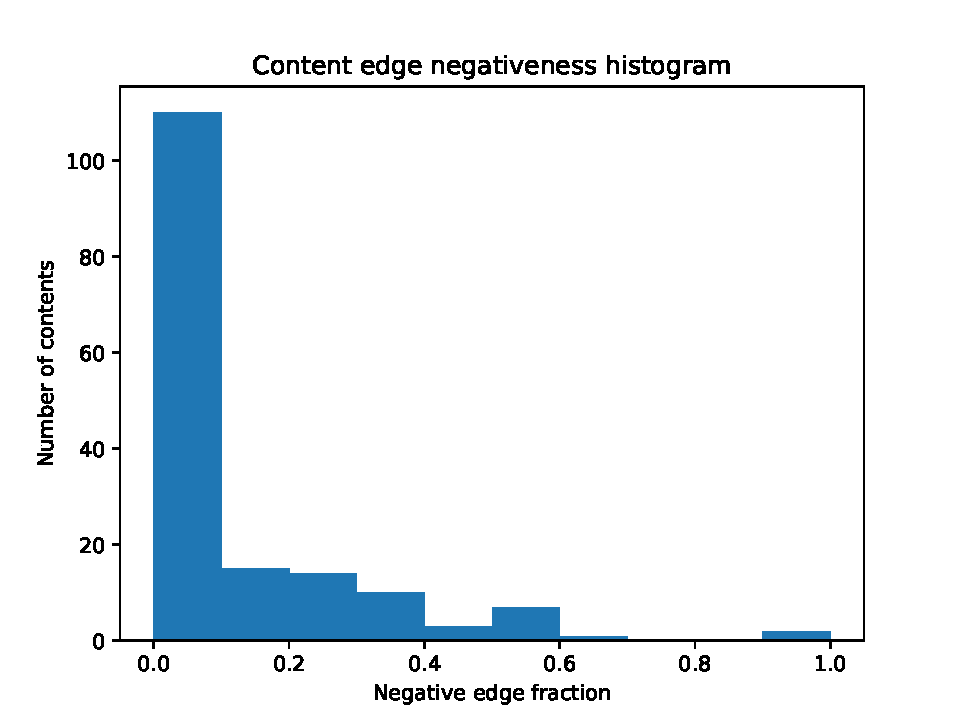
\includegraphics[width=\textwidth]{out/cats200/neg-fraction-content-hist.pdf}
				\caption{r/cats}
				\label{fig:out/bbcscience200/neg-fraction-content-hist.pdf}
			\end{subfigure}
			\begin{subfigure}[b]{0.4\textwidth}
				\centering
				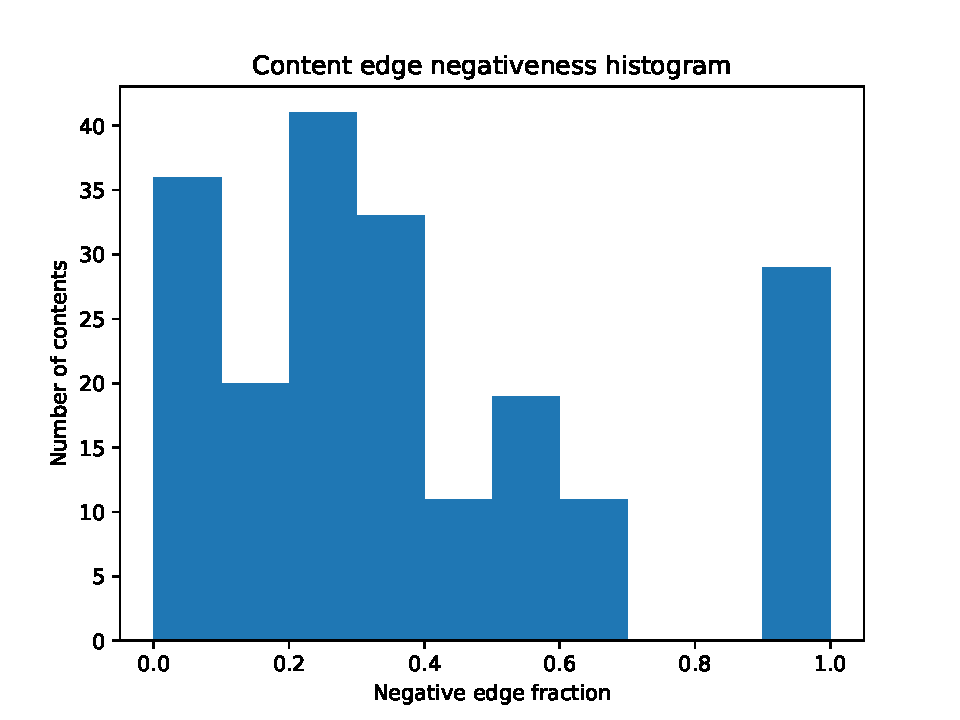
\includegraphics[width=\textwidth]{out/covid19200/neg-fraction-content-hist.pdf}
				\caption{r/covid19}
				\label{fig:out/covid19200/neg-fraction-content-hist.pdf}
			\end{subfigure}
			\begin{subfigure}[b]{0.4\textwidth}
				\centering
				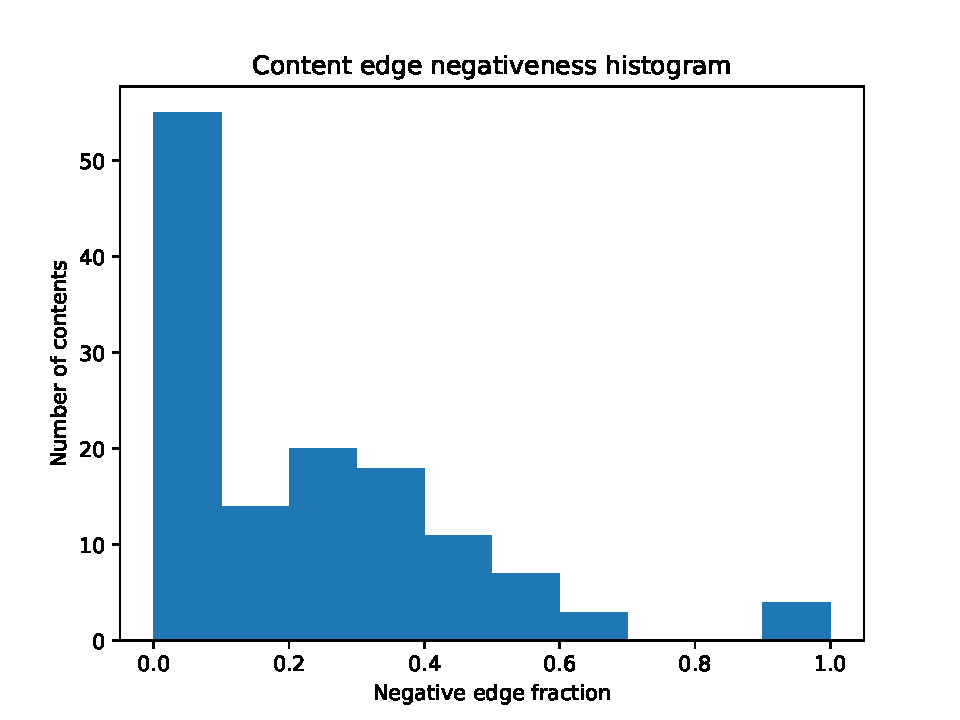
\includegraphics[width=\textwidth]{out/programming200/neg-fraction-content-hist.pdf}
				\caption{r/programming}
				\label{fig:out/bbcscience200/neg-fraction-content-hist.pdf}
			\end{subfigure}
			\begin{subfigure}[b]{0.4\textwidth}
				\centering
				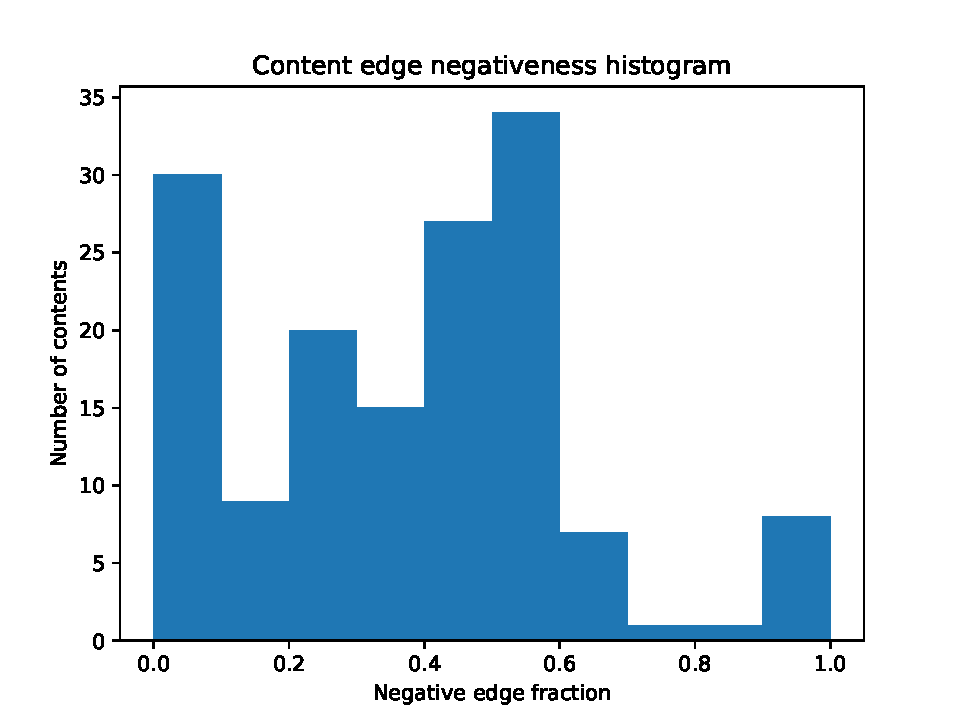
\includegraphics[width=\textwidth]{out/climate200/neg-fraction-content-hist.pdf}
				\caption{r/climate}
				\label{fig:out/bbctech200/neg-fraction-content-hist.pdf}
			\end{subfigure}
		\end{center}
	\end{figure}

\end{frame}

\begin{frame}[c]
	\frametitle{The datasets - negative edge fractions for contents}
	\begin{figure}
		\begin{center}
			\begin{subfigure}[b]{0.4\textwidth}
				\centering
				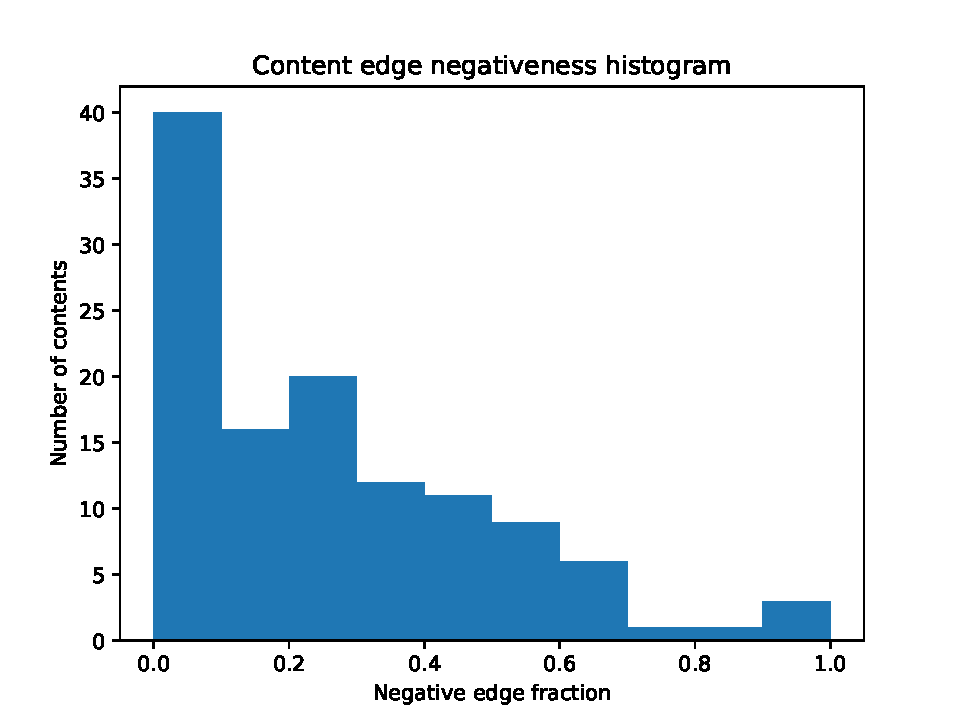
\includegraphics[width=\textwidth]{out/football200/neg-fraction-content-hist.pdf}
				\caption{r/football}
				\label{fig:out/bbcscience200/neg-fraction-content-hist.pdf}
			\end{subfigure}
			\begin{subfigure}[b]{0.4\textwidth}
				\centering
				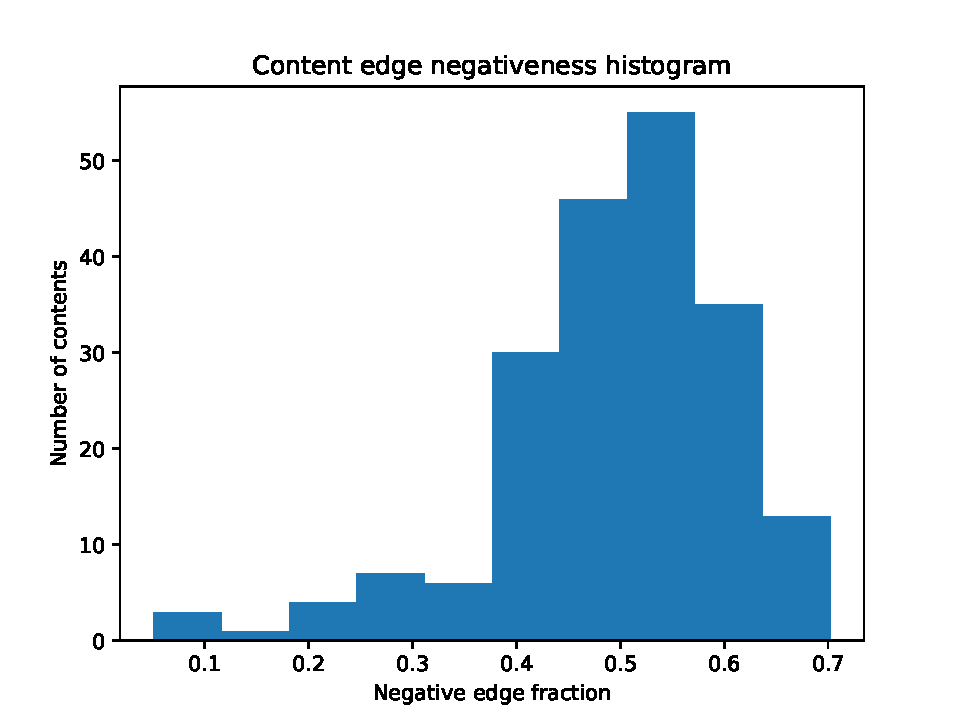
\includegraphics[width=\textwidth]{out/asktrumpsupporters200/neg-fraction-content-hist.pdf}
				\caption{r/asktrumpsupporters}
				\label{fig:out/covid19200/neg-fraction-content-hist.pdf}
			\end{subfigure}
			\begin{subfigure}[b]{0.4\textwidth}
				\centering
				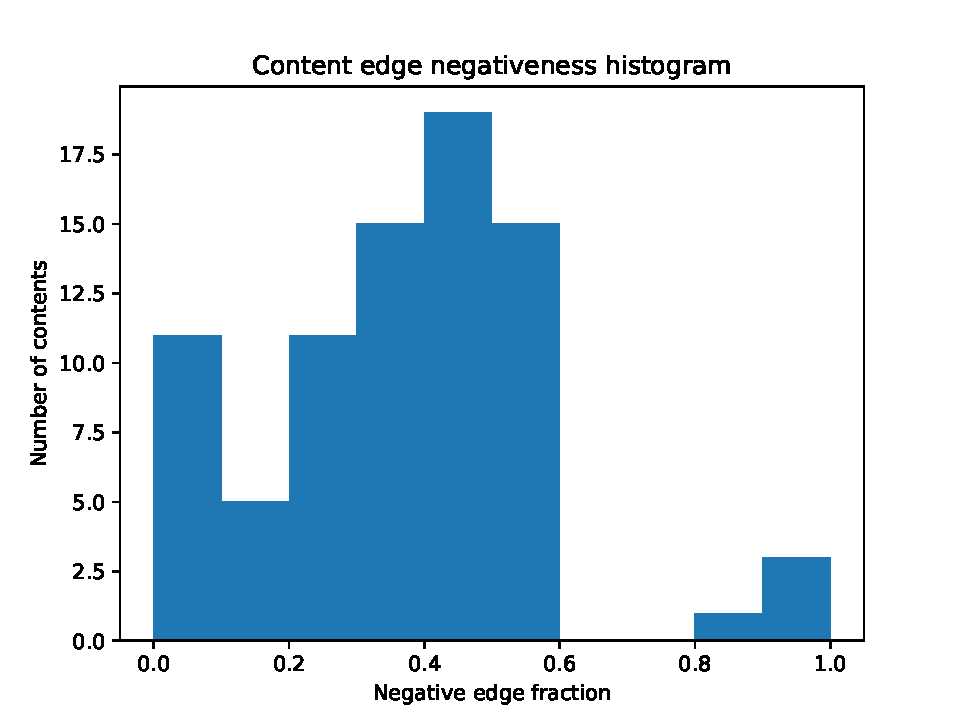
\includegraphics[width=\textwidth]{out/economics200/neg-fraction-content-hist.pdf}
				\caption{r/economics}
				\label{fig:out/bbcscience200/neg-fraction-content-hist.pdf}
			\end{subfigure}
			\begin{subfigure}[b]{0.4\textwidth}
				\centering
				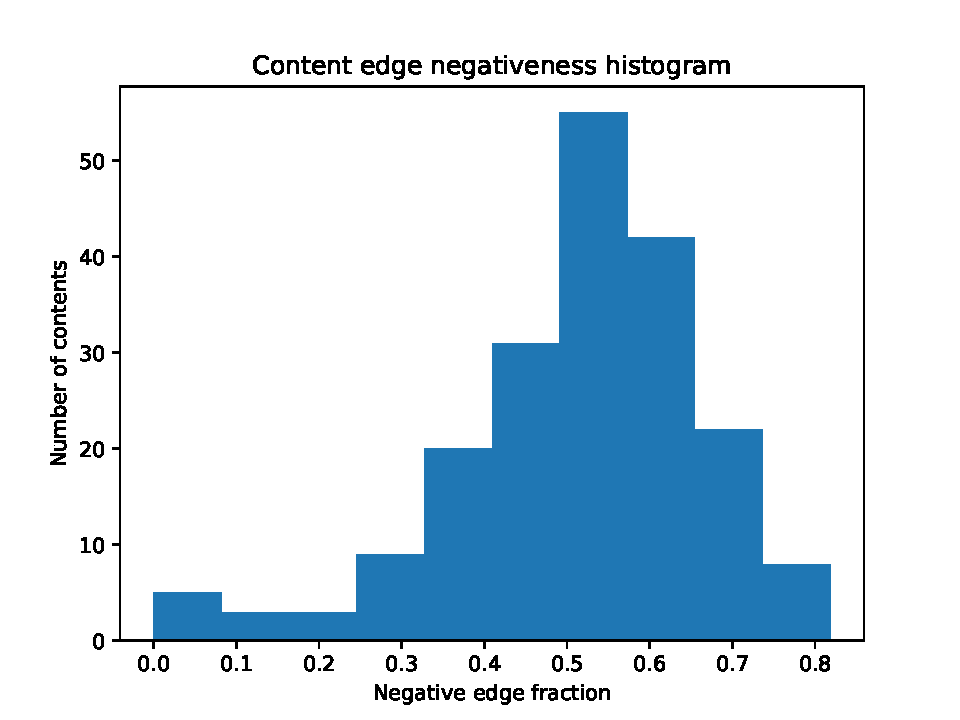
\includegraphics[width=\textwidth]{out/politics200/neg-fraction-content-hist.pdf}
				\caption{r/politics}
				\label{fig:out/bbctech200/neg-fraction-content-hist.pdf}
			\end{subfigure}
		\end{center}
	\end{figure}

\end{frame}

\begin{frame}[c]
	\frametitle{Results}

	\tiny{
		\begin{table}[htpb]
			\centering
			\caption{Echo chamber scores. For the $\xi_{round}(G) $ the results tuple
				corresponds to (score, $|U|$, number of contributing threads, time in
				seconds). In the other scores the number of contributing thread
				is omitted. $\alpha = 0.4$}
			\begin{tabular}{c|c|c|c}
				\textbf{Source, $|V|$, $|E|$, $|\hat{\mathcal{C}}  |$} & $\xi_{round}(G) $          & $\psi_{Dens}(G)$ & $\psi_{T-Dest} (G)$ \\
				\hline
				cats, 2162, 2866, 11                                   & (16, 27, 4, 1)             & (0.75, 7, 12)    & (0.75, 16, 12)      \\
				covid19, 2595, 5806, 65                                & (295, 216, 28, 4)          & (1.14, 7, 17)    & (1.57, 16, 17)      \\
				programming, 3728, 6453, 25                            & (836, 572, 36, 10)         & (0.92, 15, 34)   & (0.92, 15, 34)      \\
				climate, 6457, 13150, 74                               & (2719, 1488, 140, 102)     & (1.30, 20, 102)  & (4.5, 2, 105)       \\
				football, 6407, 10498, 28                              & (3147, 1774, 43, 125)      & (1, 9, 102)      & (1, 9, 104)         \\
				asktrumpsupporters, 8316, 62449, 172                   & (8716, 3023, 100, 29741)   & (5.3, 185, 173)  & (12, 2, 179)        \\
				economics, 9871, 19281, 36                             & (9545, 4915, 85, 1042)     & (1.44, 29, 241)  & (1.47, 37, 247)     \\
				politics, 28695,  59334, 159                           & (36696, 17420, 243, 16438) & (2.49, 55, 1967) & (5.33, 3, 1940)     \\
			\end{tabular}
		\end{table}
	}

\end{frame}

\begin{frame}[c]
	\frametitle{A solvable Densest Echo Chamber problem (3)}
	Other alternatives:

	\begin{itemize}
		\item Compute DCS-** on $G$, where each snapshot corresponds to a
		      content
		      \begin{itemize}
			      \item DCS-MM and DCS-MA trivially 0 due to sparseness
			      \item DCS-AA equivalent to previous measure
			      \item DCS-AM very close to 0 due to sparseness
		      \end{itemize}

		\item Solve O$^{2} \textsc{Bff}$ problem on the preprocessed graph
		      sequence, i.e.

		      \bigskip

		      \emph{Given a graph history $\mathcal{G}  = \{G_1 , G_2, . . . ,
				      G_{\tau}  \}$, an aggregate density function $f$ , and an
			      integer $k$, find a subset of nodes $S \subseteq V$ , and a
			      subset $\mathcal{C} _{k} $ of $\mathcal{G} $ of size $k$,
			      such that $f (S, C_k )$ is maximized}

		      \bigskip

		      O$^{2} \textsc{Bff}$-AM can be computed and more meaningful for a
		      good choice of $k$.
	\end{itemize}
\end{frame}

\begin{frame}[c]
	\frametitle{A model for the Echo Chamber Problem (1)}
	Model parameters:
	\begin{itemize}
		\item $b_{i} $, the group of each user $i$
		\item $\omega ^{+} _{rs} $ and $\omega ^{-} _{rs} $, the probabilities
		      of positive and negative edges, respectively, between users in
		      group $r$ and $s$ ($\omega ^{+} _{rs} + \omega ^{-} _{rs} \leq 1$).
		\item $\theta$, controlling the reduction of probability of interacting
		      between \emph{inactive} communities
	\end{itemize}

	For each content:
	\begin{enumerate}
		\item Sample $n'$ among the $n$ communities. These are the
		      \emph{active} communities in the content discussion
		\item For each node pairing $i, j$ consider their corresponding groups $r$ and
		      $s$.
		      \begin{itemize}
			      \item If both communities are \emph{active} draw from the
			            categorical distribution $(\omega _{rs} ^{+}, \omega
				            _{rs} ^{-}, 1 - \omega _{rs} ^{+} - \omega _{rs} ^{-}) $ to add an edge (or
			            not).
			      \item Otherwise draw from the categorical $(\theta \omega _{rs} ^{+},
				            \theta \omega
				            _{rs} ^{-}, 1 - \theta (\omega _{rs} ^{+} + \omega _{rs}
				            ^{-}))$, $\theta \leq 1$.
		      \end{itemize}

	\end{enumerate}

\end{frame}

\begin{frame}[c]
	\frametitle{A model for the Echo Chamber Problem (2)}
	Again each node has a group assignment and there are probabilities of
	positive and negative edges $\omega _{rs}^{+}  $ and $\omega _{rs}^{+}  $,
	respectively.

	\begin{enumerate}
		\item Generate the \emph{follow} graph $G$ by using a SBM with parameters
		      $\{ \phi _{rs}  \}$.
		\item Each node can be active with probability $\beta_{a}  $
		\item Any active node activates his inactive neighbours in $G$ with
		      probability $\beta_n$
		      % \item Let $a_{i} $ be the number of \emph{active} neighbours of node
		      %     $i$ in $G$ and $m_{i} $ the number of neighbours of node $i$ in
		      %     $G$. Any node inactive from the previous step is activated with
		      %     probability $ \frac{a_i}{m_i} \beta _{n} $
		\item active nodes interact according to the categorical $(\omega _{rs}
			      ^{+}, \omega _{rs} ^{-}, 1 - \omega _{rs} ^{+} - \omega _{rs} ^{-})
		      $ otherwise (at least one of the 2 nodes is inactive) with
		      categorical $(\theta \omega _{rs} ^{+}, \theta \omega _{rs} ^{-}, 1
			      - \theta (\omega _{rs} ^{+} + \omega _{rs} ^{-}))$, $\theta \leq 1$
	\end{enumerate}

\end{frame}
\begin{frame}[c]
	\frametitle{Computing the score on the synthetic data (1)}
	The following results are based on the second model. Results are also
	evaluated against known nodes communities by repeatedly solving the echo
	chamber problem on the graph (from which edges contributing to the score
	are iteratively removed).

	\bigskip

	Clustering is evaluated through Rand score, i.e. the fraction of pair of
	nodes which correspond in the predicted and true clustering.
	These are:
	\begin{itemize}
		\item pairs of nodes which are in the same cluster in the predicted and
		      true clustering;
		\item pairs of nodes which are in different clusters in the predicted
		      and true clustering.
	\end{itemize}
	Also an \emph{adjusted} version of the measure is provided, comparing the
	score against a random assignment of the labels.

	\bigskip

\end{frame}

\begin{frame}[c]
	\frametitle{Computing the score on the synthetic data (2)}
	The following graphs contains 4 communities among which vertices are
	equally distributed and 10
	threads, with $\alpha = 0.2$. The results have been computed with the
	non-exact algorithm.

	\bigskip

	$\beta _{a} = 1/8, \;\beta_{n} = 1/3, \; \theta = 1/10, \; \phi = 0.7$
	(usually) for nodes inside the same community and $\phi = 0.2$ for nodes
	in different community. These parameters control graph density.
\end{frame}

\begin{frame}[c]
	\frametitle{Computing the score on the synthetic data (3)}
	First graph: clean division of communities with mainly positive edges inside the groups and negative edges between groups.

	\begin{figure}
		\begin{center}
			\begin{subfigure}[b]{0.3\textwidth}
				\centering
				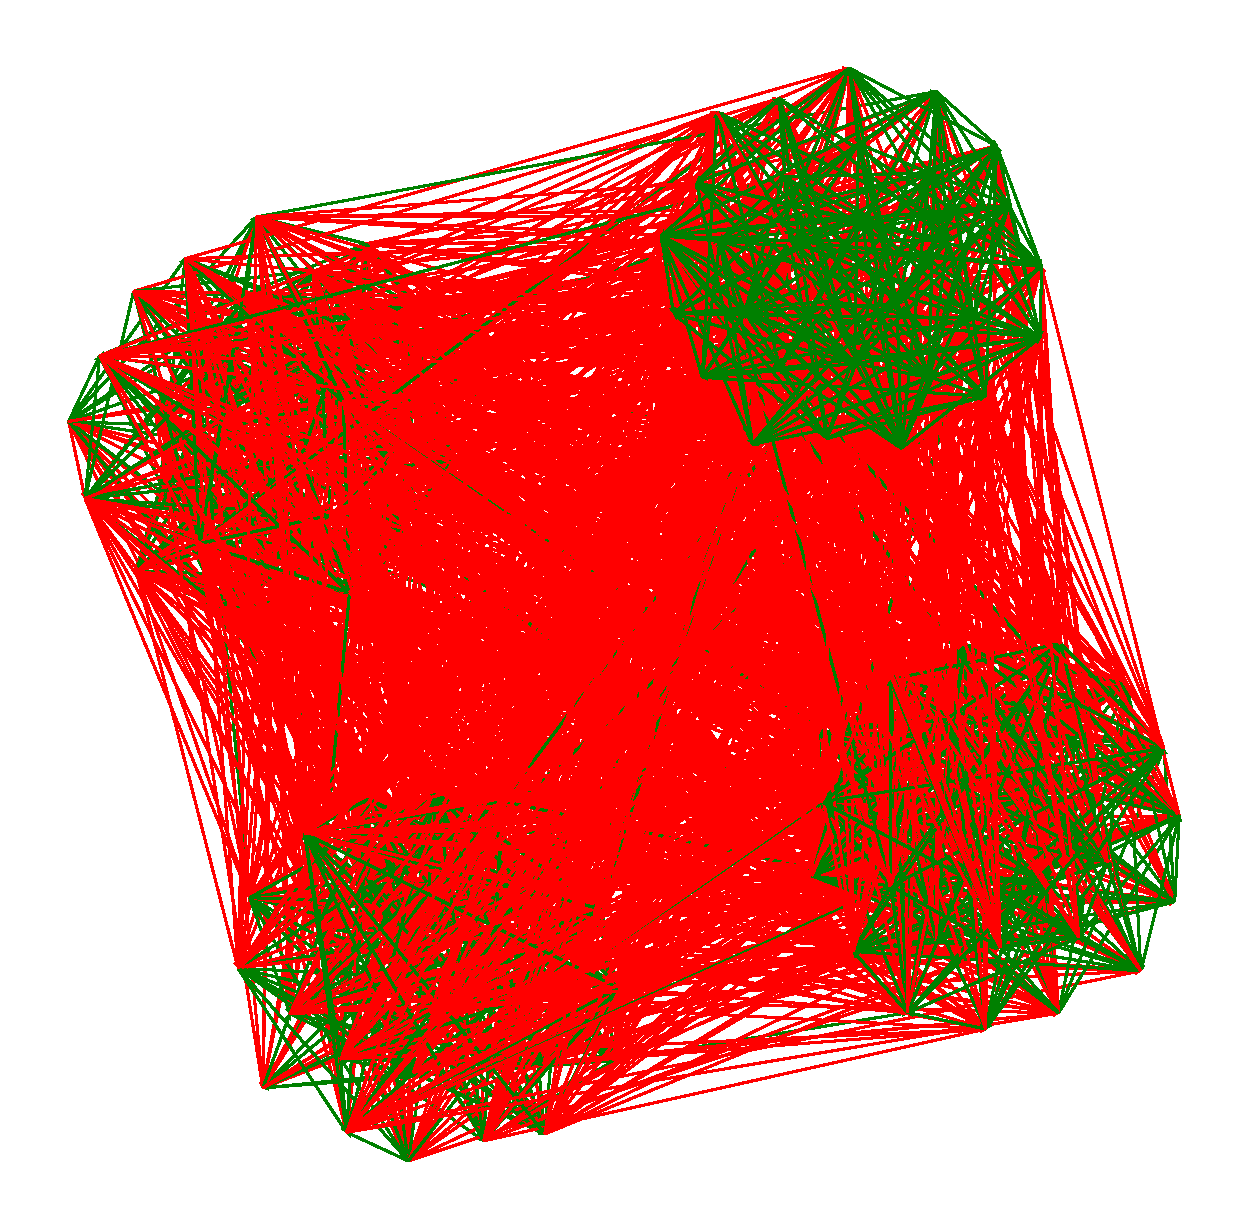
\includegraphics[width=\textwidth]{out/synthetic/model2_graph4.pdf}
				\caption{Graph}
				\label{fig:}
			\end{subfigure}
			\begin{subfigure}[b]{0.3\textwidth}
				\centering
				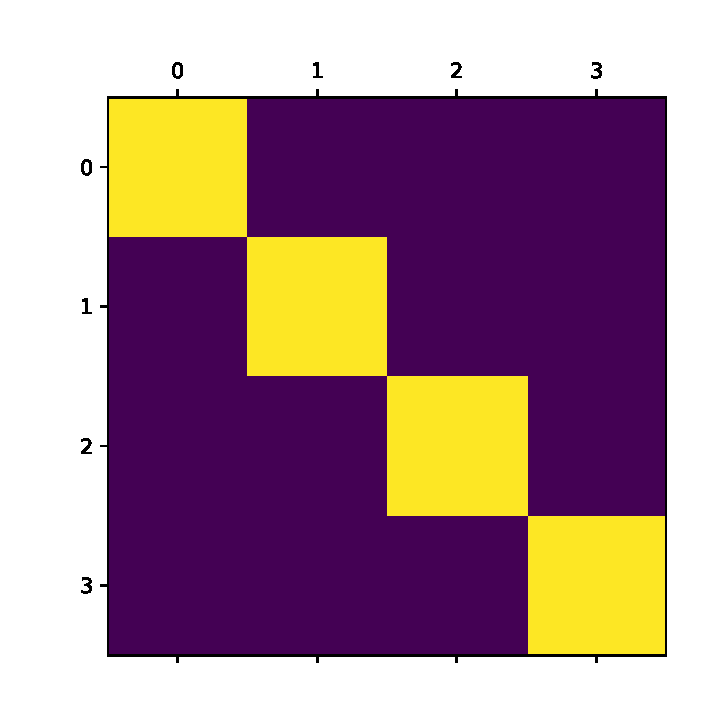
\includegraphics[width=\textwidth]{out/synthetic/model2_omega_positive4.pdf}
				\caption{$\omega ^{+} _{rs} $}
				\label{fig:out/synthetic/omega_positive1.pdf}
			\end{subfigure}
			\begin{subfigure}[b]{0.3\textwidth}
				\centering
				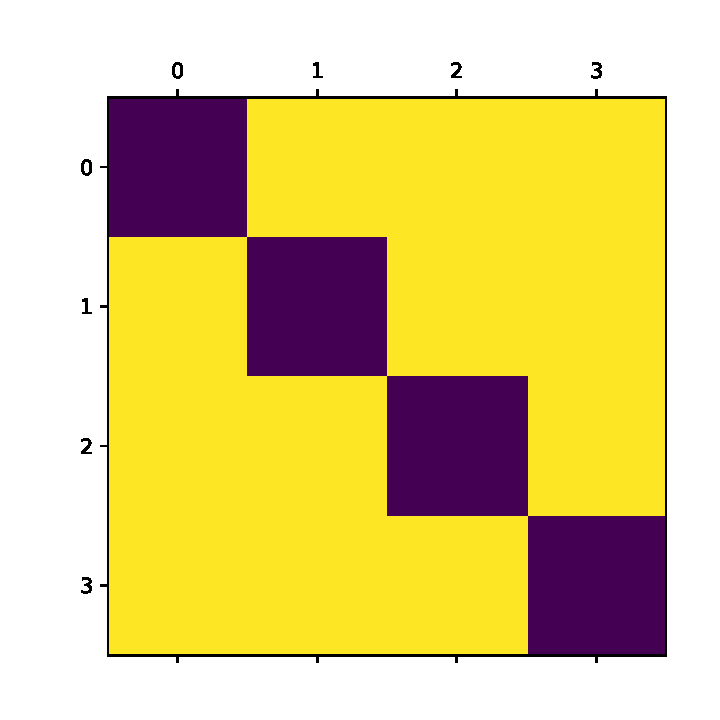
\includegraphics[width=\textwidth]{out/synthetic/model2_omega_negative4.pdf}
				\caption{$\omega ^{-} _{rs} $}
				\label{fig:}
			\end{subfigure}
		\end{center}
	\end{figure}

	$|V| = 120, \; |E| \approx 2400, \; \eta(G) \approx 0.6, \; \bar{\xi}(G)
		\approx 91$.

	Rand $= 0.7$, adjusted Rand $= 0.25$
	% Time (single iteration): $8.5 $ seconds.
\end{frame}

\begin{frame}[c]
	\frametitle{Computing the score on the synthetic data (4)}
	Second graph: much smaller distinction in the interaction between
	communities.

	\begin{figure}
		\begin{center}
			\begin{subfigure}[b]{0.3\textwidth}
				\centering
				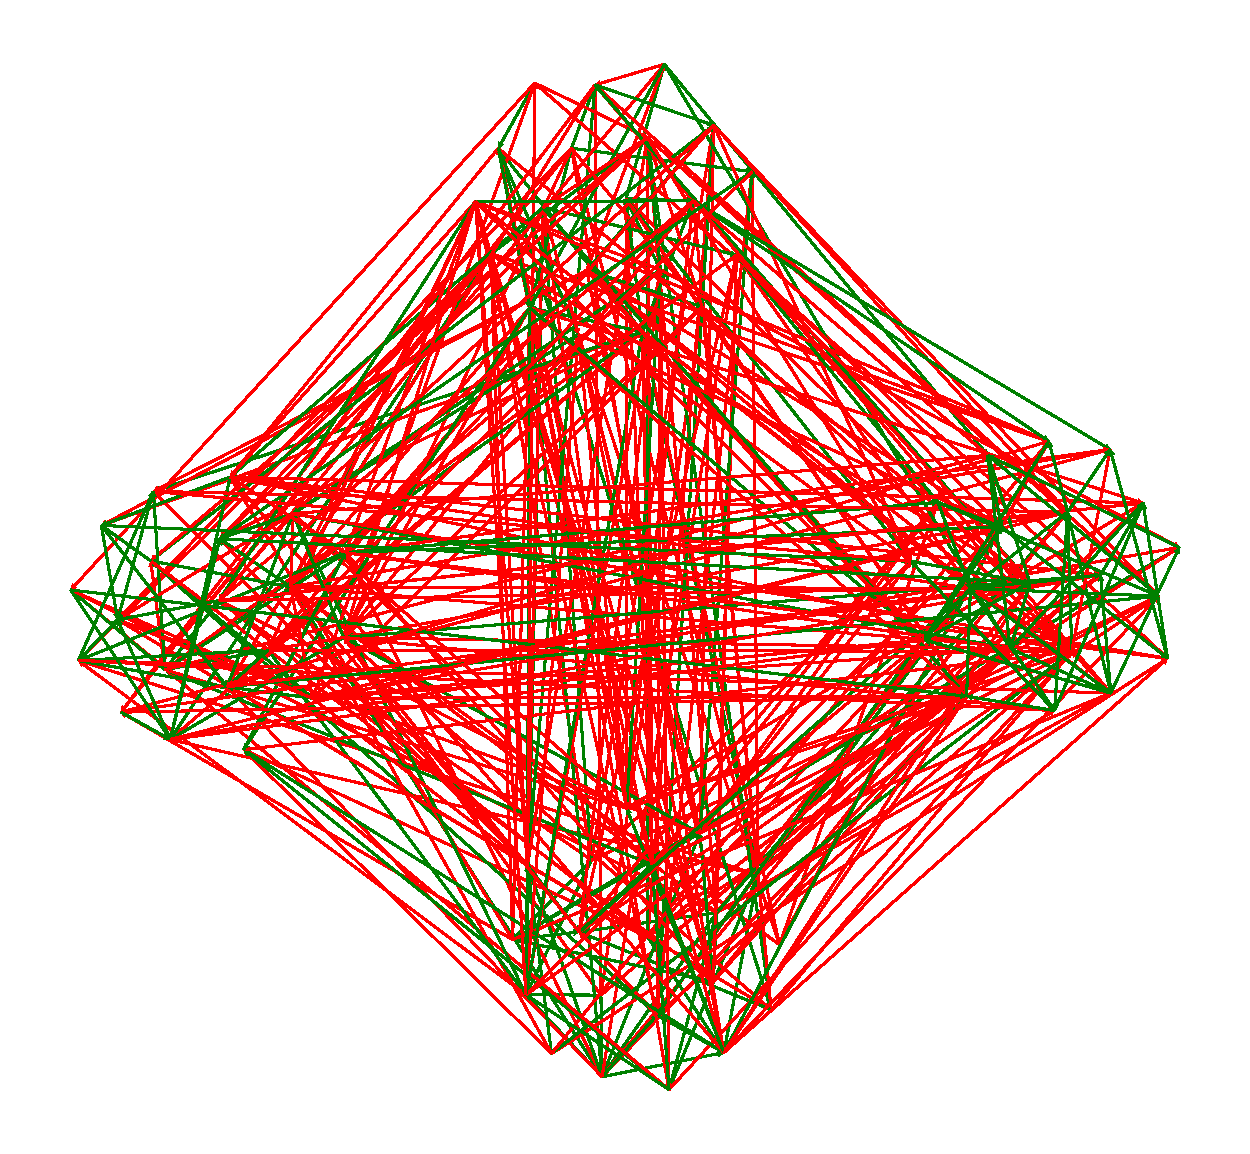
\includegraphics[width=\textwidth]{out/synthetic/model2_graph1.pdf}
				\caption{Graph}
				\label{fig:}
			\end{subfigure}
			\begin{subfigure}[b]{0.3\textwidth}
				\centering
				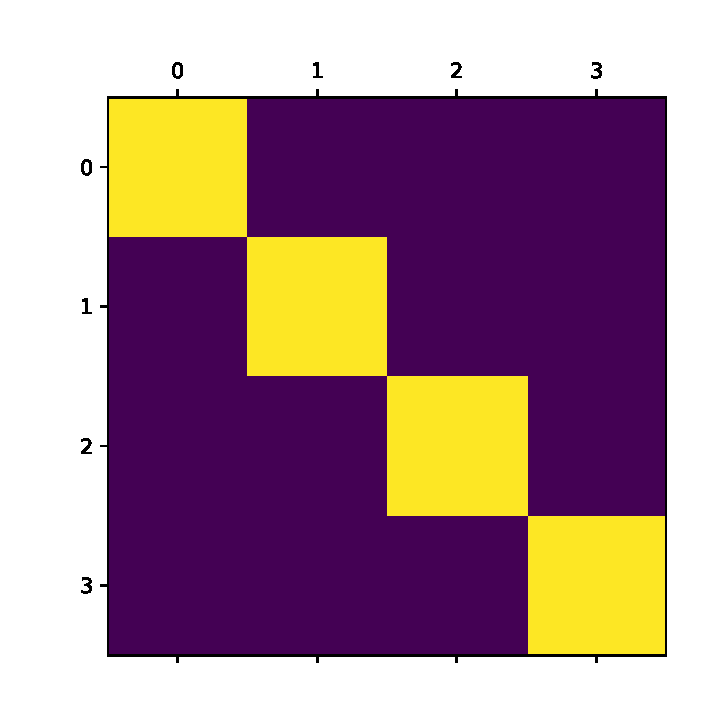
\includegraphics[width=\textwidth]{out/synthetic/model2_omega_positive2.pdf}
				\caption{$\omega ^{+} _{rs} $}
				\label{fig:out/synthetic/omega_positive1.pdf}
			\end{subfigure}
			\begin{subfigure}[b]{0.3\textwidth}
				\centering
				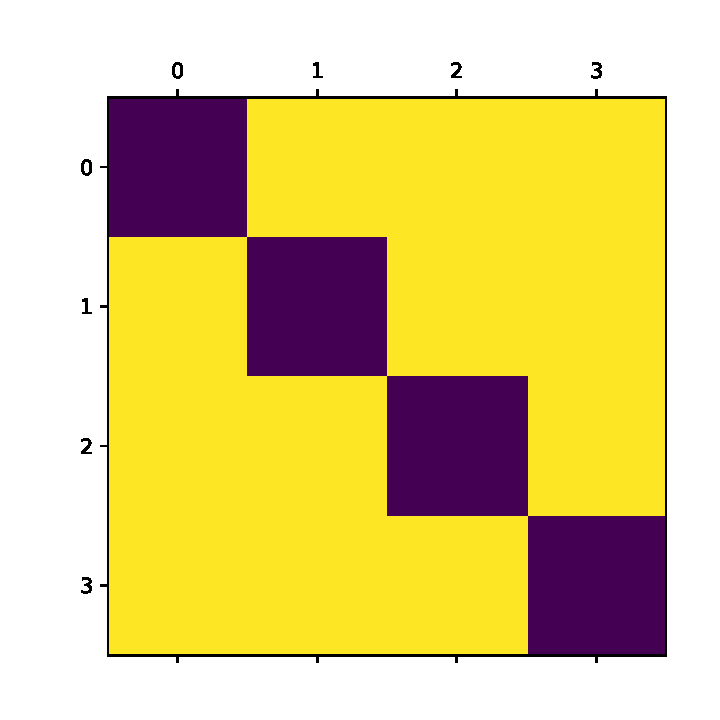
\includegraphics[width=\textwidth]{out/synthetic/model2_omega_negative2.pdf}
				\caption{$\omega ^{-} _{rs} $}
				\label{fig:}
			\end{subfigure}
		\end{center}
	\end{figure}

	$|V| = 80, \; |E| \approx 400, \; \eta(G) \approx 0.7, \; \bar{\xi}(G)
		\approx 16$.

	Rand $= 0.6$, adjusted Rand $= 0.026$
\end{frame}

\begin{frame}[c]
	\frametitle{Computing the score on the synthetic data (5)}
	Third graph: much smaller distinction in the interaction between
	communities.

	\begin{figure}
		\begin{center}
			\begin{subfigure}[b]{0.3\textwidth}
				\centering
				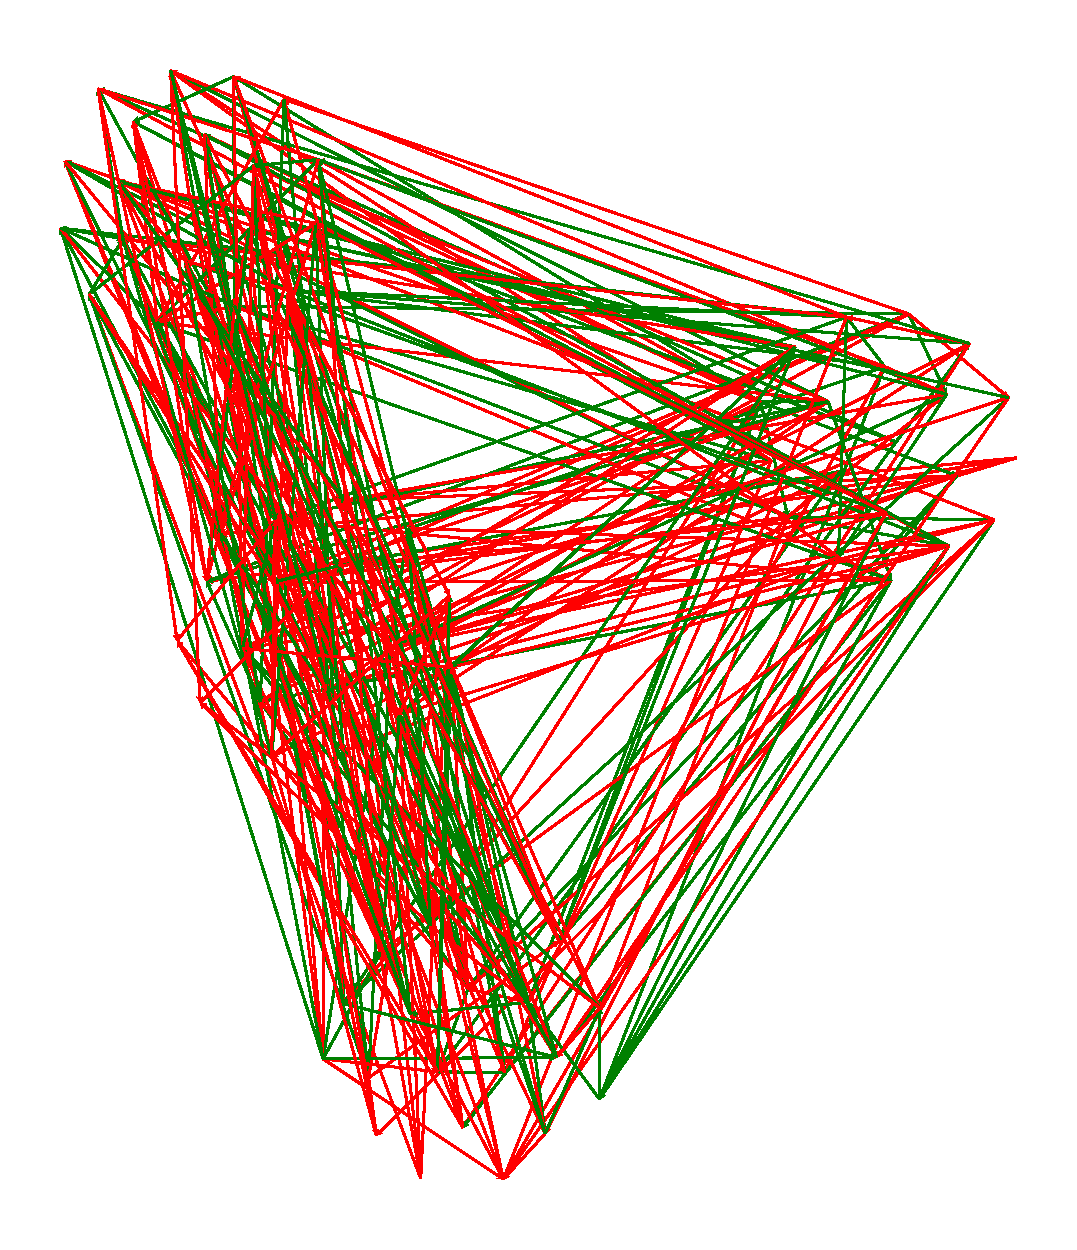
\includegraphics[width=\textwidth]{out/synthetic/model2_graph2.pdf}
				\caption{Graph}
				\label{fig:}
			\end{subfigure}
			\begin{subfigure}[b]{0.3\textwidth}
				\centering
				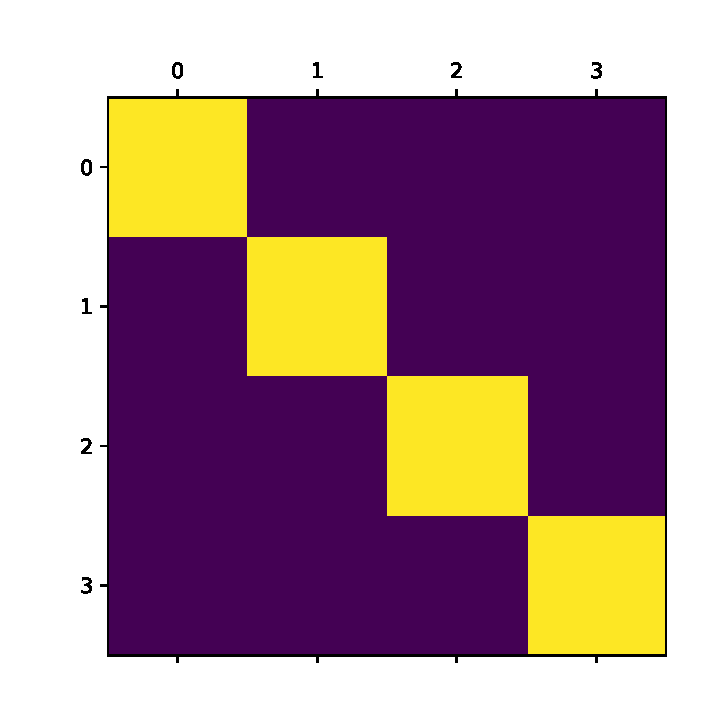
\includegraphics[width=\textwidth]{out/synthetic/model2_omega_positive3.pdf}
				\caption{$\omega ^{+} _{rs} $}
				\label{fig:out/synthetic/omega_positive1.pdf}
			\end{subfigure}
			\begin{subfigure}[b]{0.3\textwidth}
				\centering
				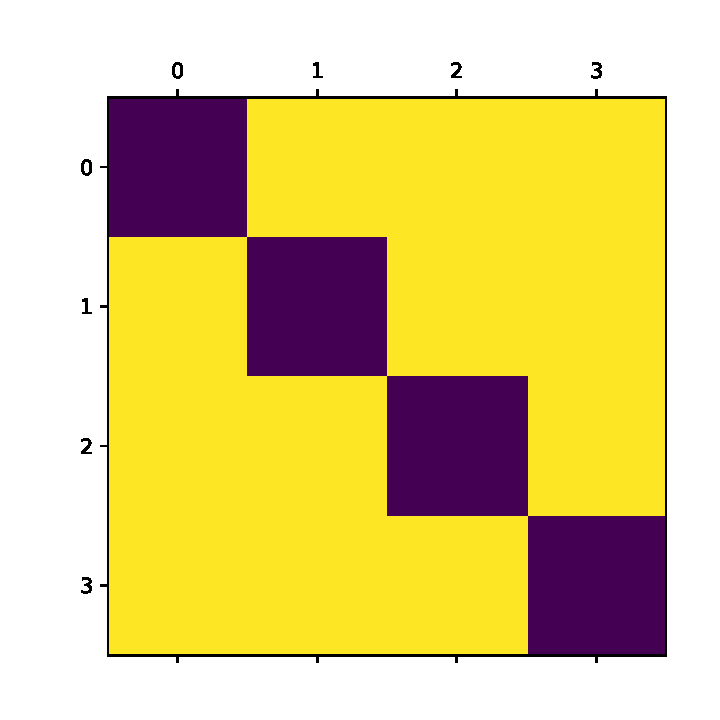
\includegraphics[width=\textwidth]{out/synthetic/model2_omega_negative3.pdf}
				\caption{$\omega ^{-} _{rs} $}
				\label{fig:}
			\end{subfigure}
		\end{center}
	\end{figure}

	$|V| = 80, \; |E| \approx 400, \; \eta(G) \approx 0.58, \; \bar{\xi}(G)
		\approx 25$.

	Rand $= 0.6$, adjusted Rand $= 0.007$
\end{frame}

\begin{frame}[c]
	\frametitle{Observations on the result}
	\begin{itemize}
		\item Increasing the number of vertices in each community helps
		      clustering correcly the nodes
		\item the lower the distiction of interactions between communities,
		      the more it is difficult to find a correct clustering
		\item in order to find a good clustering $\alpha $ may be chosen to
		      be equal to the $\eta$ inside each of the communities, so that a
		      single whole community does not produce many controversial
		      threads in the induced subgraphs
	\end{itemize}
\end{frame}

\end{document}
